\section{Прогнозирование временных рядов}

\subsection{Временные ряды}

Временным рядом называется последовательность значений признака y, измеряемого 
через постоянные временные интервалы:

\begin{equation*}
    y_1, \dots, y_T, \dots, \quad y_t \in \mathbb{R}.
\end{equation*}
В этом определении нужно обратить внимание на то, что временные интервалы между 
измерениями признака постоянны.\\[-0.5em]

\begin{figure}[h!]
    \centering
    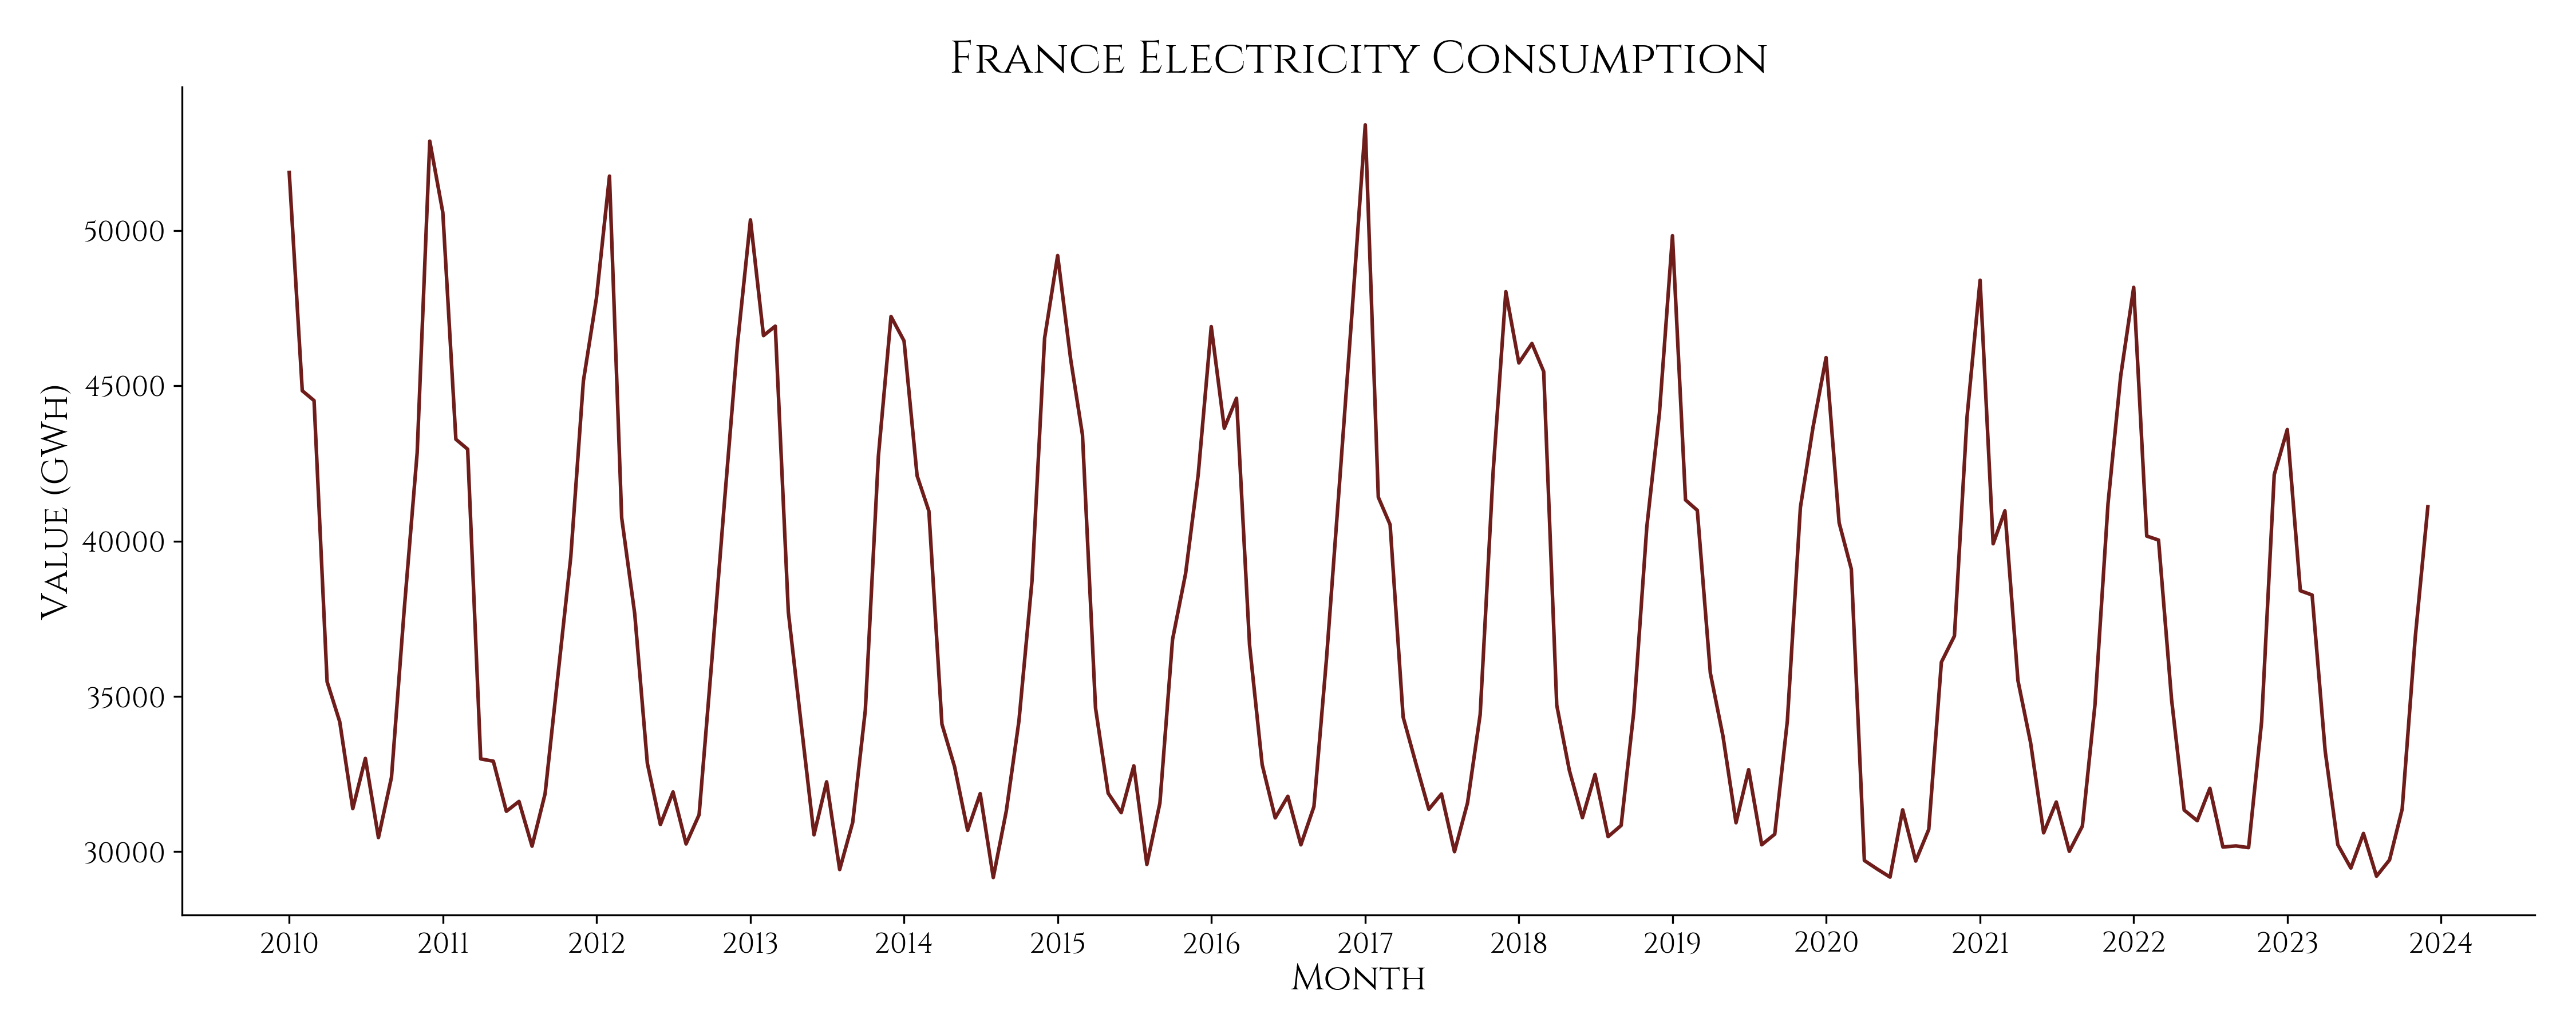
\includegraphics[width=1\textwidth, height=1\textheight, keepaspectratio]{time_series_example_France}
    \caption{Ежемесячное потребление электричества во Франции. 
    Построено программой по адресу (листинг \ref{lst:time_series_example_France}).}
    \label{fig:time_series_example_France}
\end{figure}

Временные ряды изобилуют в таких
областях, как экономика, бизнес, инженерия, естественные науки 
(особенно геофизика и метеорология), а также социальные науки.

Примеры временных рядов - это ряды с  
ежемесячной последовательностью объемов отгруженных с завода товаров, 
еженедельными данными о количестве дорожно-транспортных происшествий, 
ежедневными объемами осадков, почасовыми наблюдениями за химическеми 
выбросами. Ещё один пример временного ряда 
(показан на рисунке \ref{fig:time_series_example_France}) — это реальное 
ежемесячное потребление электричества во Франции.

\subsubsection{Прогнозирование временного ряда \cite{TSA_Box}}

Информация о доступных наблюдениях в момент времени $t$ временного ряда, 
используемая для предсказания его значения в некотором будущем $t+l$ может 
предоставить фундамент для планирования в бизнесе и экономике, контроля продукции, 
оптимизации индустриальных процессов и так далее. Здесь $l$ - это, так называемый, 
\textit{горизонт прогнозирования}, который меняется от задачи к задаче.

Предположим, что наблюдения - \textit{дискретные}, равноудаленные друг от друга величины. 
Например в задаче прогнозирования продаж, продажи $z_t$ в текущий месяц $t$ и продажи 
$z_{t-1}, z_{t-2}, z_{t-3}, ...$ в предыдущие месяцы можно использовать для 
прогнозирования горизонта в $l = 1, 2, 3, ..., 12$ месяцев. Обозначим за $\hat{z}_t (l)$ 
прогноз, составленный в \textit{момент времени} $t$ для продаж $z_{t+l}$ в некотором будущем $t+l$, т.е.
с \textit{горизонтом прогнозирования} $l$. Функция $\hat{z}_t (l)$, прогнозирующая в момент времени 
$t$ для всех будущих горизнтов прогнозирования, на основе доступной информации о 
текущем и предыдущих значениях $z_t, z_{t-1}, z_{t-2}, z_{t-3}, ...$ на протяжении времени $t$, 
называется \textit{функцией прогнозирования} в момент времени $t$. Основная задача 
прогнозирования временных рядов заключается в том, чтобы найти функцию прогнозирования с 
наименьшим средним квадратом отклонений $z_{t+l} - \hat{z}_t (l)$ между истинными и 
спрогнозированными значениями для каждого из \textit{горизонтов прогнозирования} $l$. 

В добавок к нахождению наилучших прогнозов, также необходимо указать их точность, так 
чтобы, например, можно было рассчитать риски, ассоциированные с решениями, принятыми на 
их основе. Точность прогнозов можно выразить в качестве \textit{доверительных интервалов} 
с каждой стороны прогноза. Эти интервалы могут быть рассчитаны для любого удобного набора 
вероятностей, например, 50 и 95\%. Они указывают вероятность попадания спрогнозированной 
величины в данный интервал. За иллюстрацией обратимся к рис. \ref{fig:time_series_forecast_probability_limit}, 
на котором изображены последние 20 значений временного ряда, кульминирующие в момент времени $t$. 
Также представлены прогнозы, сделанные в момент времени $t$ с горизонтами прогнозирования 
$l = 1, 2, ..., 13$, вместе с 50\% доверетильными интервалами.

\begin{figure}[h!]
    \centering
    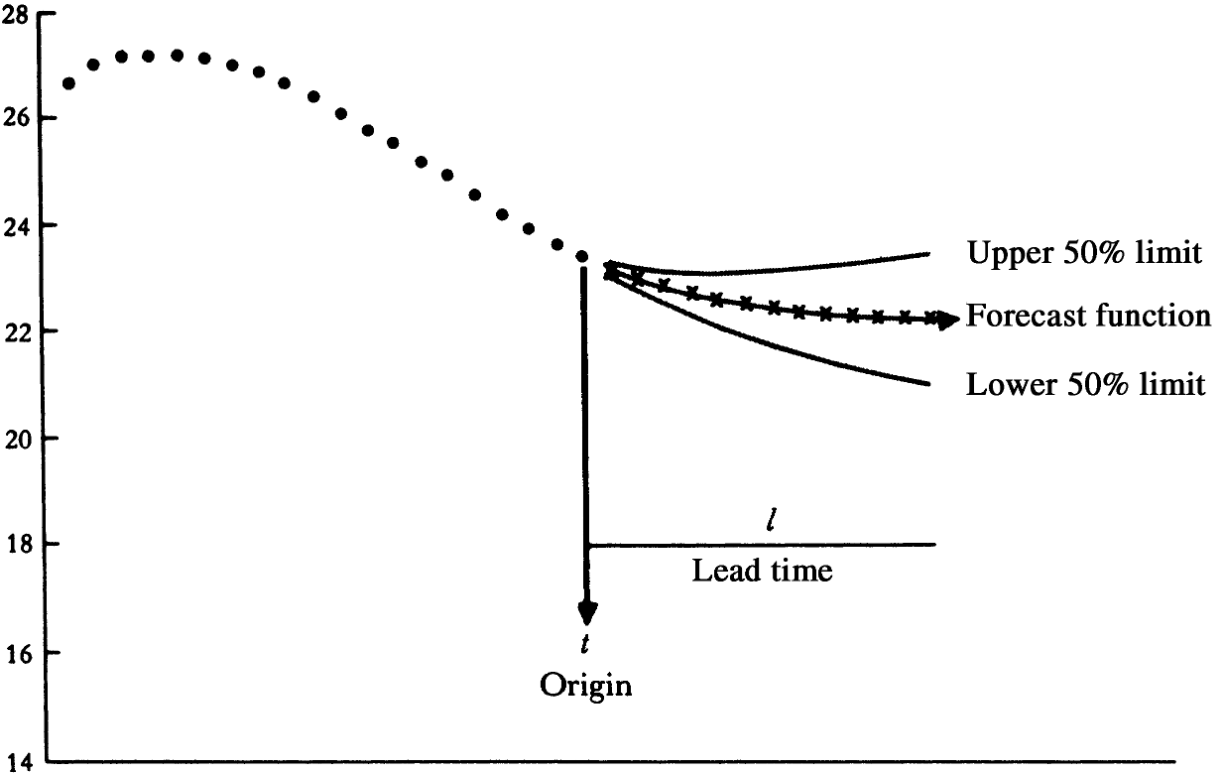
\includegraphics[width=0.8\textwidth, height=0.8\textheight, keepaspectratio]{time_series_forecast_probability_limit}
    \caption{Значения временного ряда с прогнозирующей функцией и 50\% доверетильными интервалами.}
    \label{fig:time_series_forecast_probability_limit}
\end{figure}

\subsubsection{Главная особенность временных рядов}

Чаcто, в задачах регрессионного анализа и машинного обучения, в качестве анализируемых 
данных берутся простые выборки, построенные из независимо одинаково распредленных 
наблюдений. В задаче анализа временных рядов всё с точностью наоборот: 
предполагается, что данные в прошлом каким-то образом связаны с данными в будущем. 
Чем сильнее они связаны, тем больше имеется информации о поведении временного ряда 
в будущем и тем точнее можно сделать прогноз. 

Полезно снова рассмотреть данные о реальном ежемесячном потреблении электричества во Франции 
(рис. \ref{fig:time_series_example_France}). Видно, что на графике изображена не простая 
выборка (измерения не являются независимыми и одинаково распределёнными), а сложный, 
структурированный процесс. Выявив структуру этого процесса, можно учесть её в
прогнозирующей модели и построить действительно точный прогноз.

\subsubsection{Компоненты временных рядов}

Полезно рассмотреть несколько понятий, которыми можно описать поведение временных рядов:

\begin{itemize}
    \item Тренд — плавное долгосрочное изменение уровня ряда. Эту характеристику можно получить, наблюдая
    ряд в течение достаточно долгого времени.
    \item Сезонность — циклические изменения уровня ряда с постоянным периодом. В данных о ежемесячном 
    потреблении электричества во Франции (рис. \ref{fig:time_series_example_France}) очень хорошо видны подобные 
    сезонные колебания: признак всегда принимает максимальное значение зимой, а минимальное — летом. 
    Это легко объяснить тем, что летом электричества необходимо меньше всего, это самый тёплый сезон 
    во Франции. В целом профиль изменения потребления электричества внутри года остаётся более-менее 
    постоянным.
    \item Цикл — изменение уровня ряда с переменным периодом. Такое поведение часто встречается в рядах,
    связанных с продажами, и объясняется циклическими изменениями экономической активности. В эко-
    номике выделяют циклы длиной 4 - 5 лет, 7 - 11 лет, 45 - 50 лет и т. д. Другой пример ряда с такой
    характеристикой — это солнечная активность, которая соответствует, например, количеству солнечных
    пятен за день. Она плавно меняется с периодом, который составляет несколько лет, причём сам период
    также меняется во времени.
    \item Ошибка — непрогнозируемая случайная компонента ряда. Сюда включены все те характеристики временного ряда, 
    которые сложно измерить (например, слишком слабые).
\end{itemize}

\subsection{Автокорреляция}

Одной из важнейших характеристик временного ряда является автокорреляция. Автокорреляцией 
назвается математическая репрезентация степени \guillemotleft схожести\guillemotright {} между 
исходным рядом и его версией, сдвинутой на некоторый интервал, называемый лагом. Концептуально 
это похоже на корреляцию Пирсона между двумя временными рядами, только автокорреляция рассматривает 
один и тот же ряд дважды. \\

Стоит напомнить, что коэффициент корреляции, а значит и автокорреляции может быть равен 0 при наличии сильной, 
но нелинейной зависимости (рис. \ref{fig:non_linear_correlation_example}) \cite{pml1Book}.\\

\begin{figure}[h!]
    \centering
    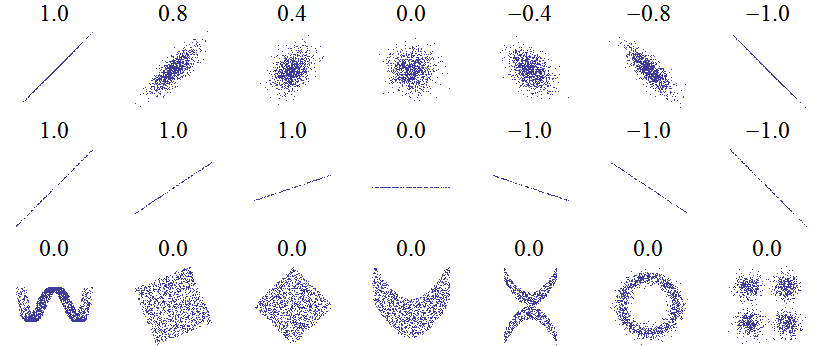
\includegraphics[width=0.9\textwidth, height=0.9\textheight, keepaspectratio]{non_linear_correlation_example}
    \caption{Несколько наборов точек (x, y) и коэффициент корреляции x и y
    для каждого набора. Отметим, что корреляция отражает зашумленность и направление 
    линейной зависимости (верхний ряд), но не отражает ее угловой
    коэффициент (средний ряд), а также многие аспекты нелинейных связей (нижний ряд). 
    (Примечание: на рисунке в центре угловой коэффициент равен 0, но
    в этом случае коэффициент корреляции не определен, потому что дисперсия Y
    нулевая.)}
    \label{fig:non_linear_correlation_example}
\end{figure}

\subsubsection{Автокорреляция, её вычисление}

Количественной характеристикой сходства между значениями ряда в соседних точках является 
автокорреляционная функция (или просто автокорреляция), которая задаётся следующим соотношением:\\

\begin{equation*}
    r_l \defeq \cfrac{\mathbb{E}[(y_t - \mathbb{E}_y)(y_{t+l} - \mathbb{E}_y)]}{\mathbb{V}_y},
\end{equation*}
где количество отсчётов, на которое сдвинут ряд, называется лагом автокорреляции $(l)$.\\
Можно заметить сходство с корреляцией Пирсона:

\begin{equation*}
    \rho \defeq \text{corr}[X, Y] \defeq 
    \cfrac{\text{Cov}[X, Y]}{\sqrt{\mathbb{V}[X]\mathbb{V}[Y]}}, \qquad 
    \text{Cov}[X, Y] \defeq \mathbb{E}[(X - \mathbb{E}[X])(Y - \mathbb{E}[Y])]
\end{equation*}

Значения, принимаемые автокорреляцией такие же, как и у коэффициента 
Пирсона: $r_l \in [-1, 1]$. Вычислить автокорреляцию по выборке можно, заменив в формуле 
математическое ожидание на выборочное среднее, а дисперсию — на выборочную дисперсию.

\subsubsection{Коррелограммы}
Анализировать величину автокорреляции при разных значениях лагов удобно с помощью графиков. 
Далее различные методы графического анализа автокорреляции будут демонстрироваться 
на примере данных о суммарном объёме продаж красного вина в Австралии за
месяц на протяжении 15 лет (рис. \ref{fig:time_series_wine}).

\begin{figure}[h!]
    \centering
    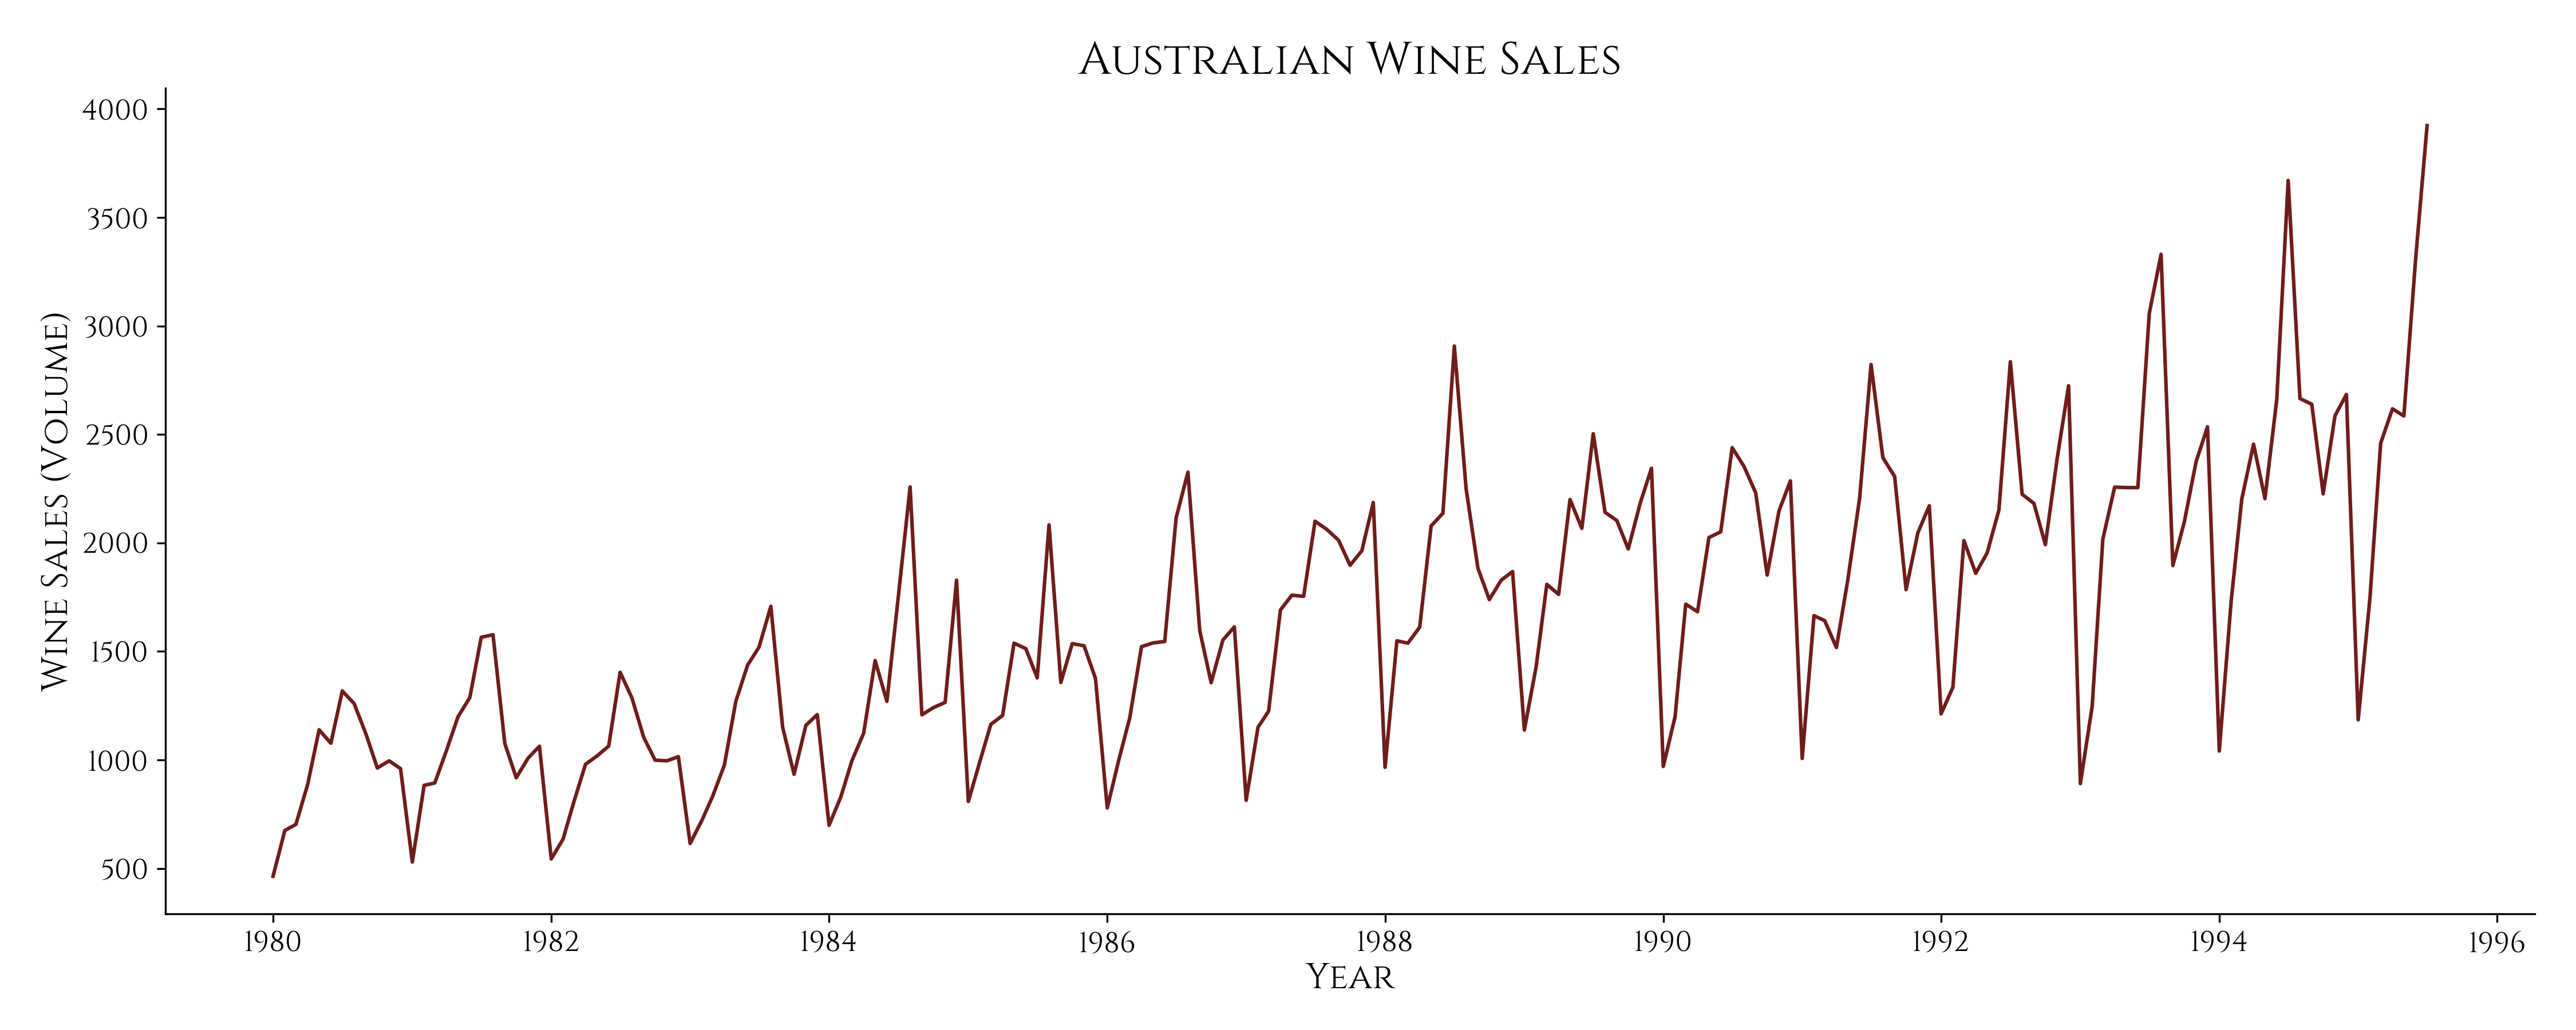
\includegraphics[width=1\textwidth, height=1\textheight, keepaspectratio]{time_series_example_wine}
    \caption{Месячный объём продаж красного вина в Австралии, в бутылках. 
    Построено программой по адресу (листинг \ref{lst:time_series_example_wine}).}
    \label{fig:time_series_wine}
\end{figure}

Этот ряд обладает ярко выраженной годовой сезонностью: максимум продаж за год 
приходится на декабрь, а затем, в январе, происходит существенное падение.

\paragraph{График задержек}
Графиком задержек (Lag Plot) называется особый вид диаграммы рассеяния (scatter plot), 
на которой по одной из ее осей откладывается значение временного ряда в момент времени 
$t$, а по другой - значение в момент времени $t + l$, где $l$ - значение лага.

\begin{center}
    \begin{minipage}{0.45\textwidth}
        \centering
        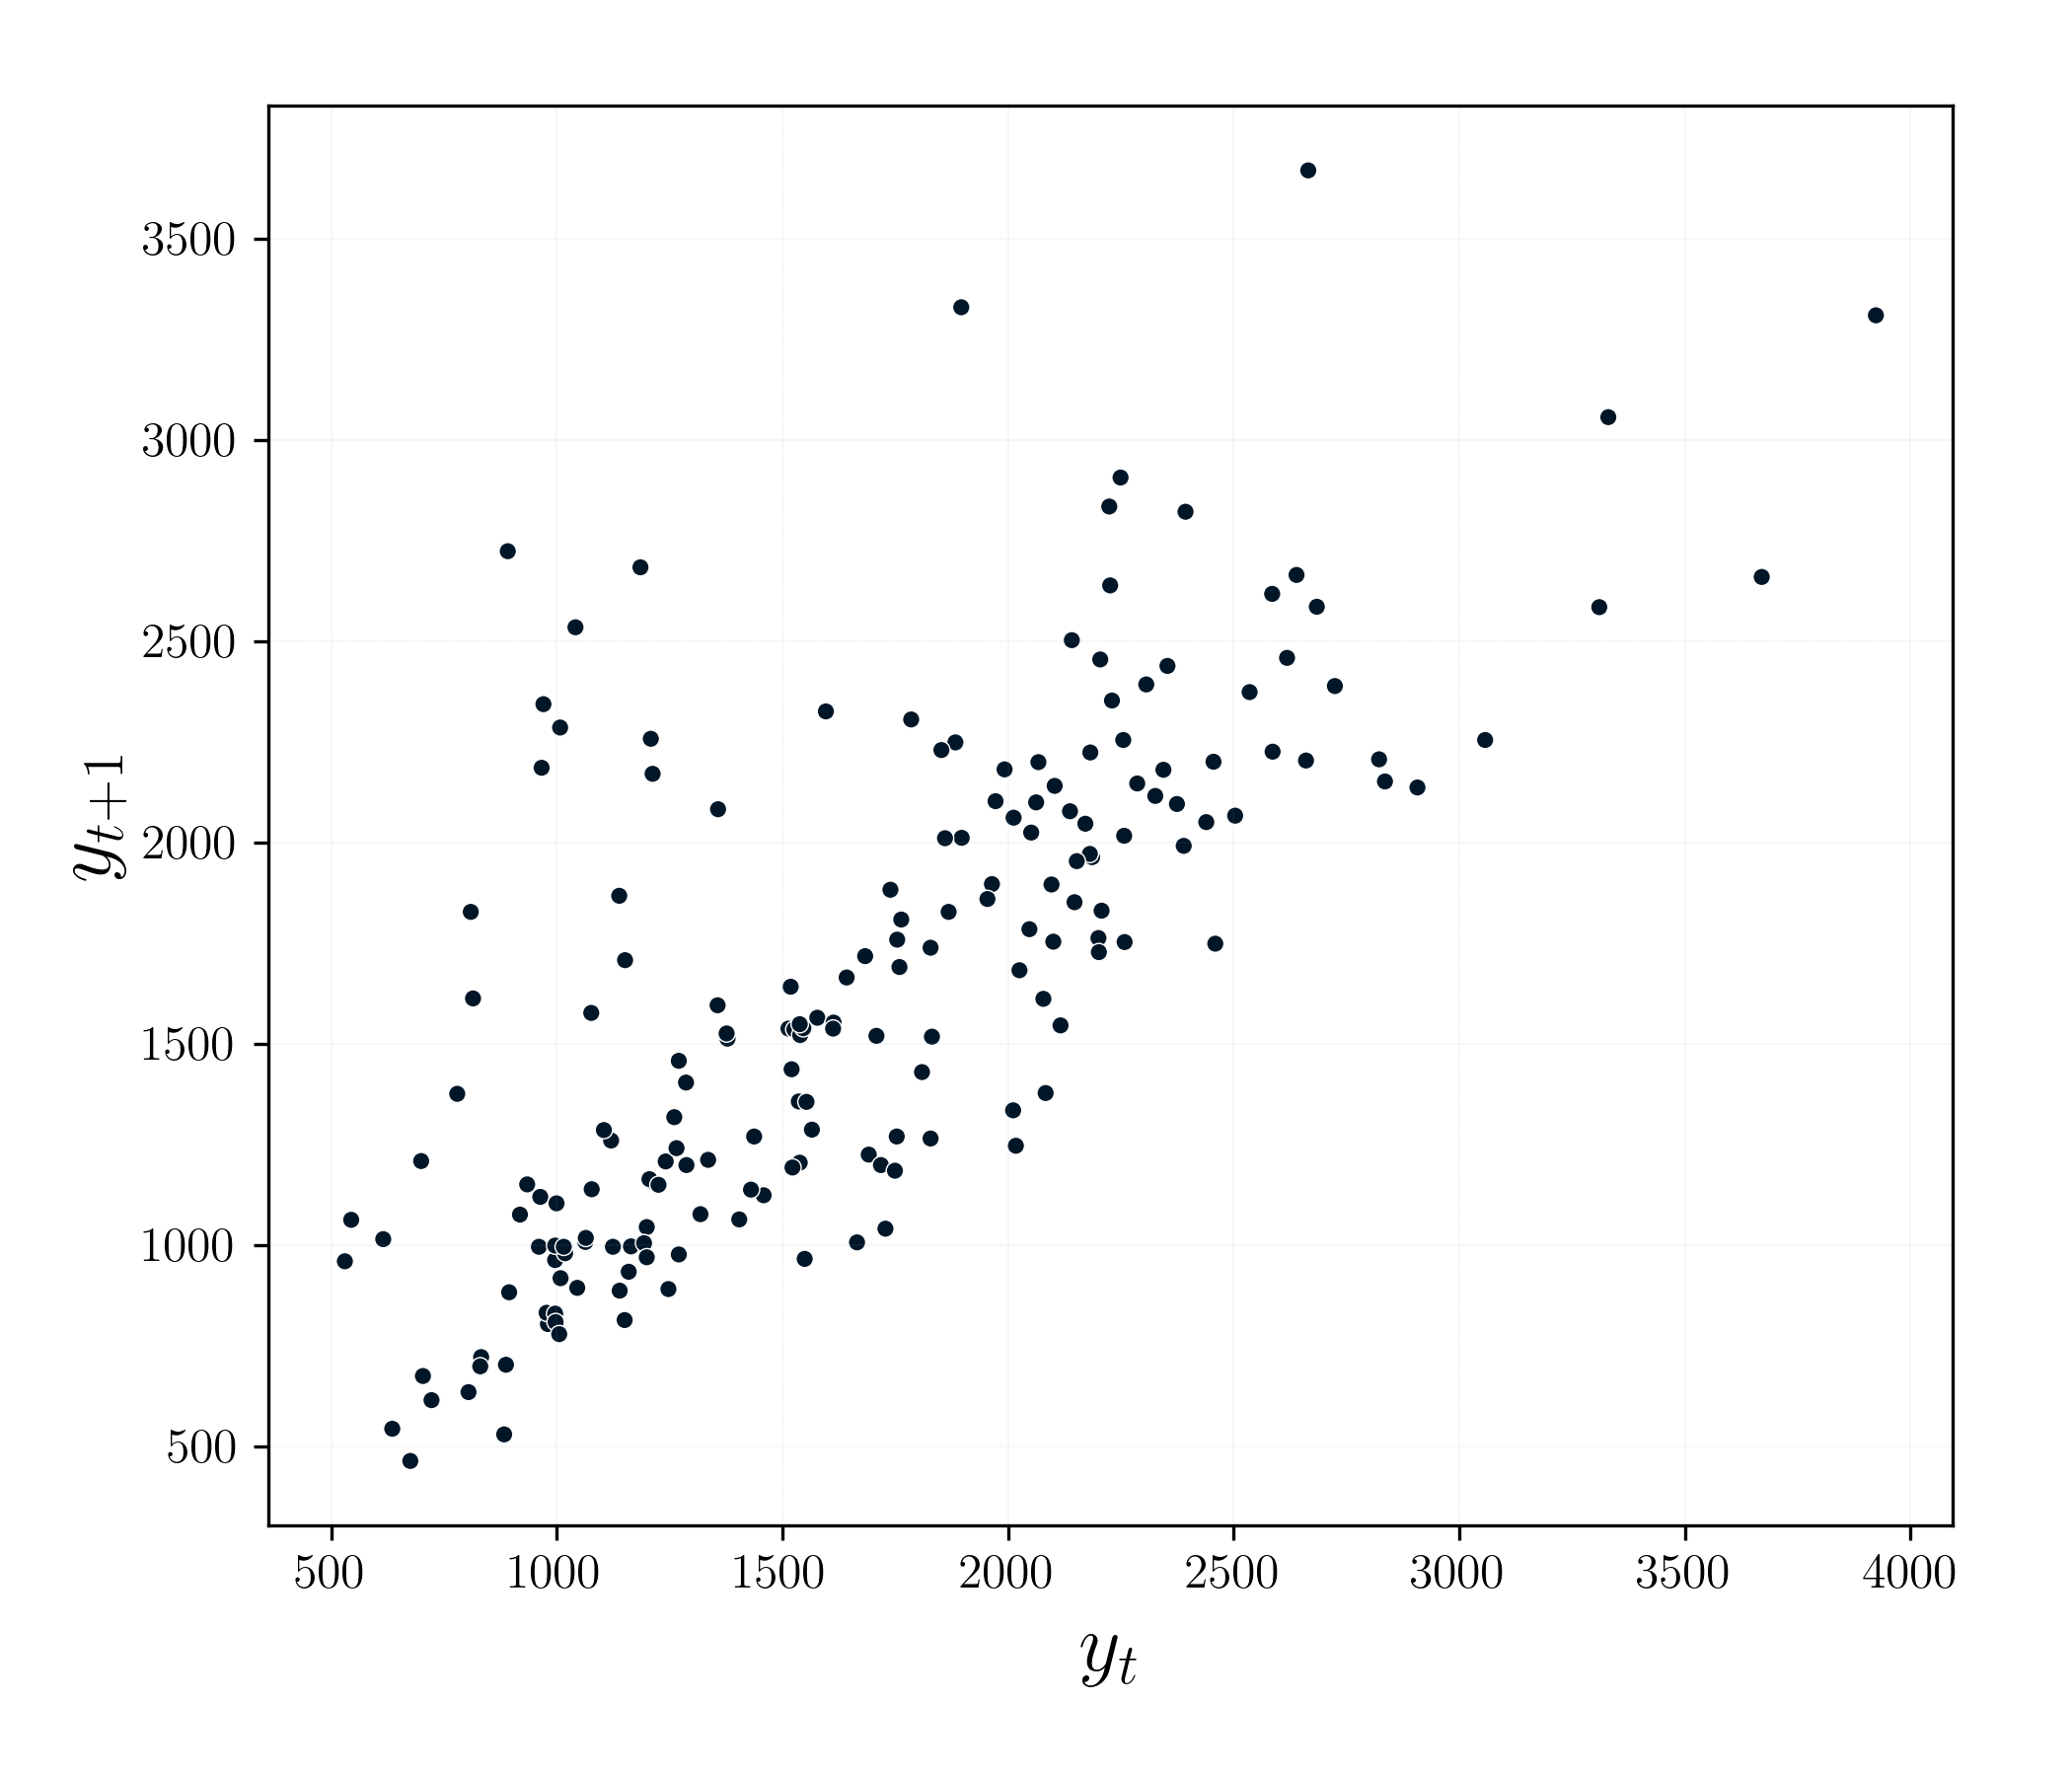
\includegraphics[width=1\textwidth, height=1\textheight, keepaspectratio]{australia_wine_lag_plot}
        \captionof{figure}{Связь между значениями объёма продаж красного вина в соседние месяцы, 
        по горизонтали отложен объём продаж в месяц t, по вертикали — в следующий месяц, 
        t + 1. Построено программой по адресу 
        (листинг \ref{lst:time_series_lag_plot_wine}).}
        \label{fig:lag_plot_wine}
    \end{minipage}
    \hfill
    \begin{minipage}{0.45\textwidth}
        \centering
        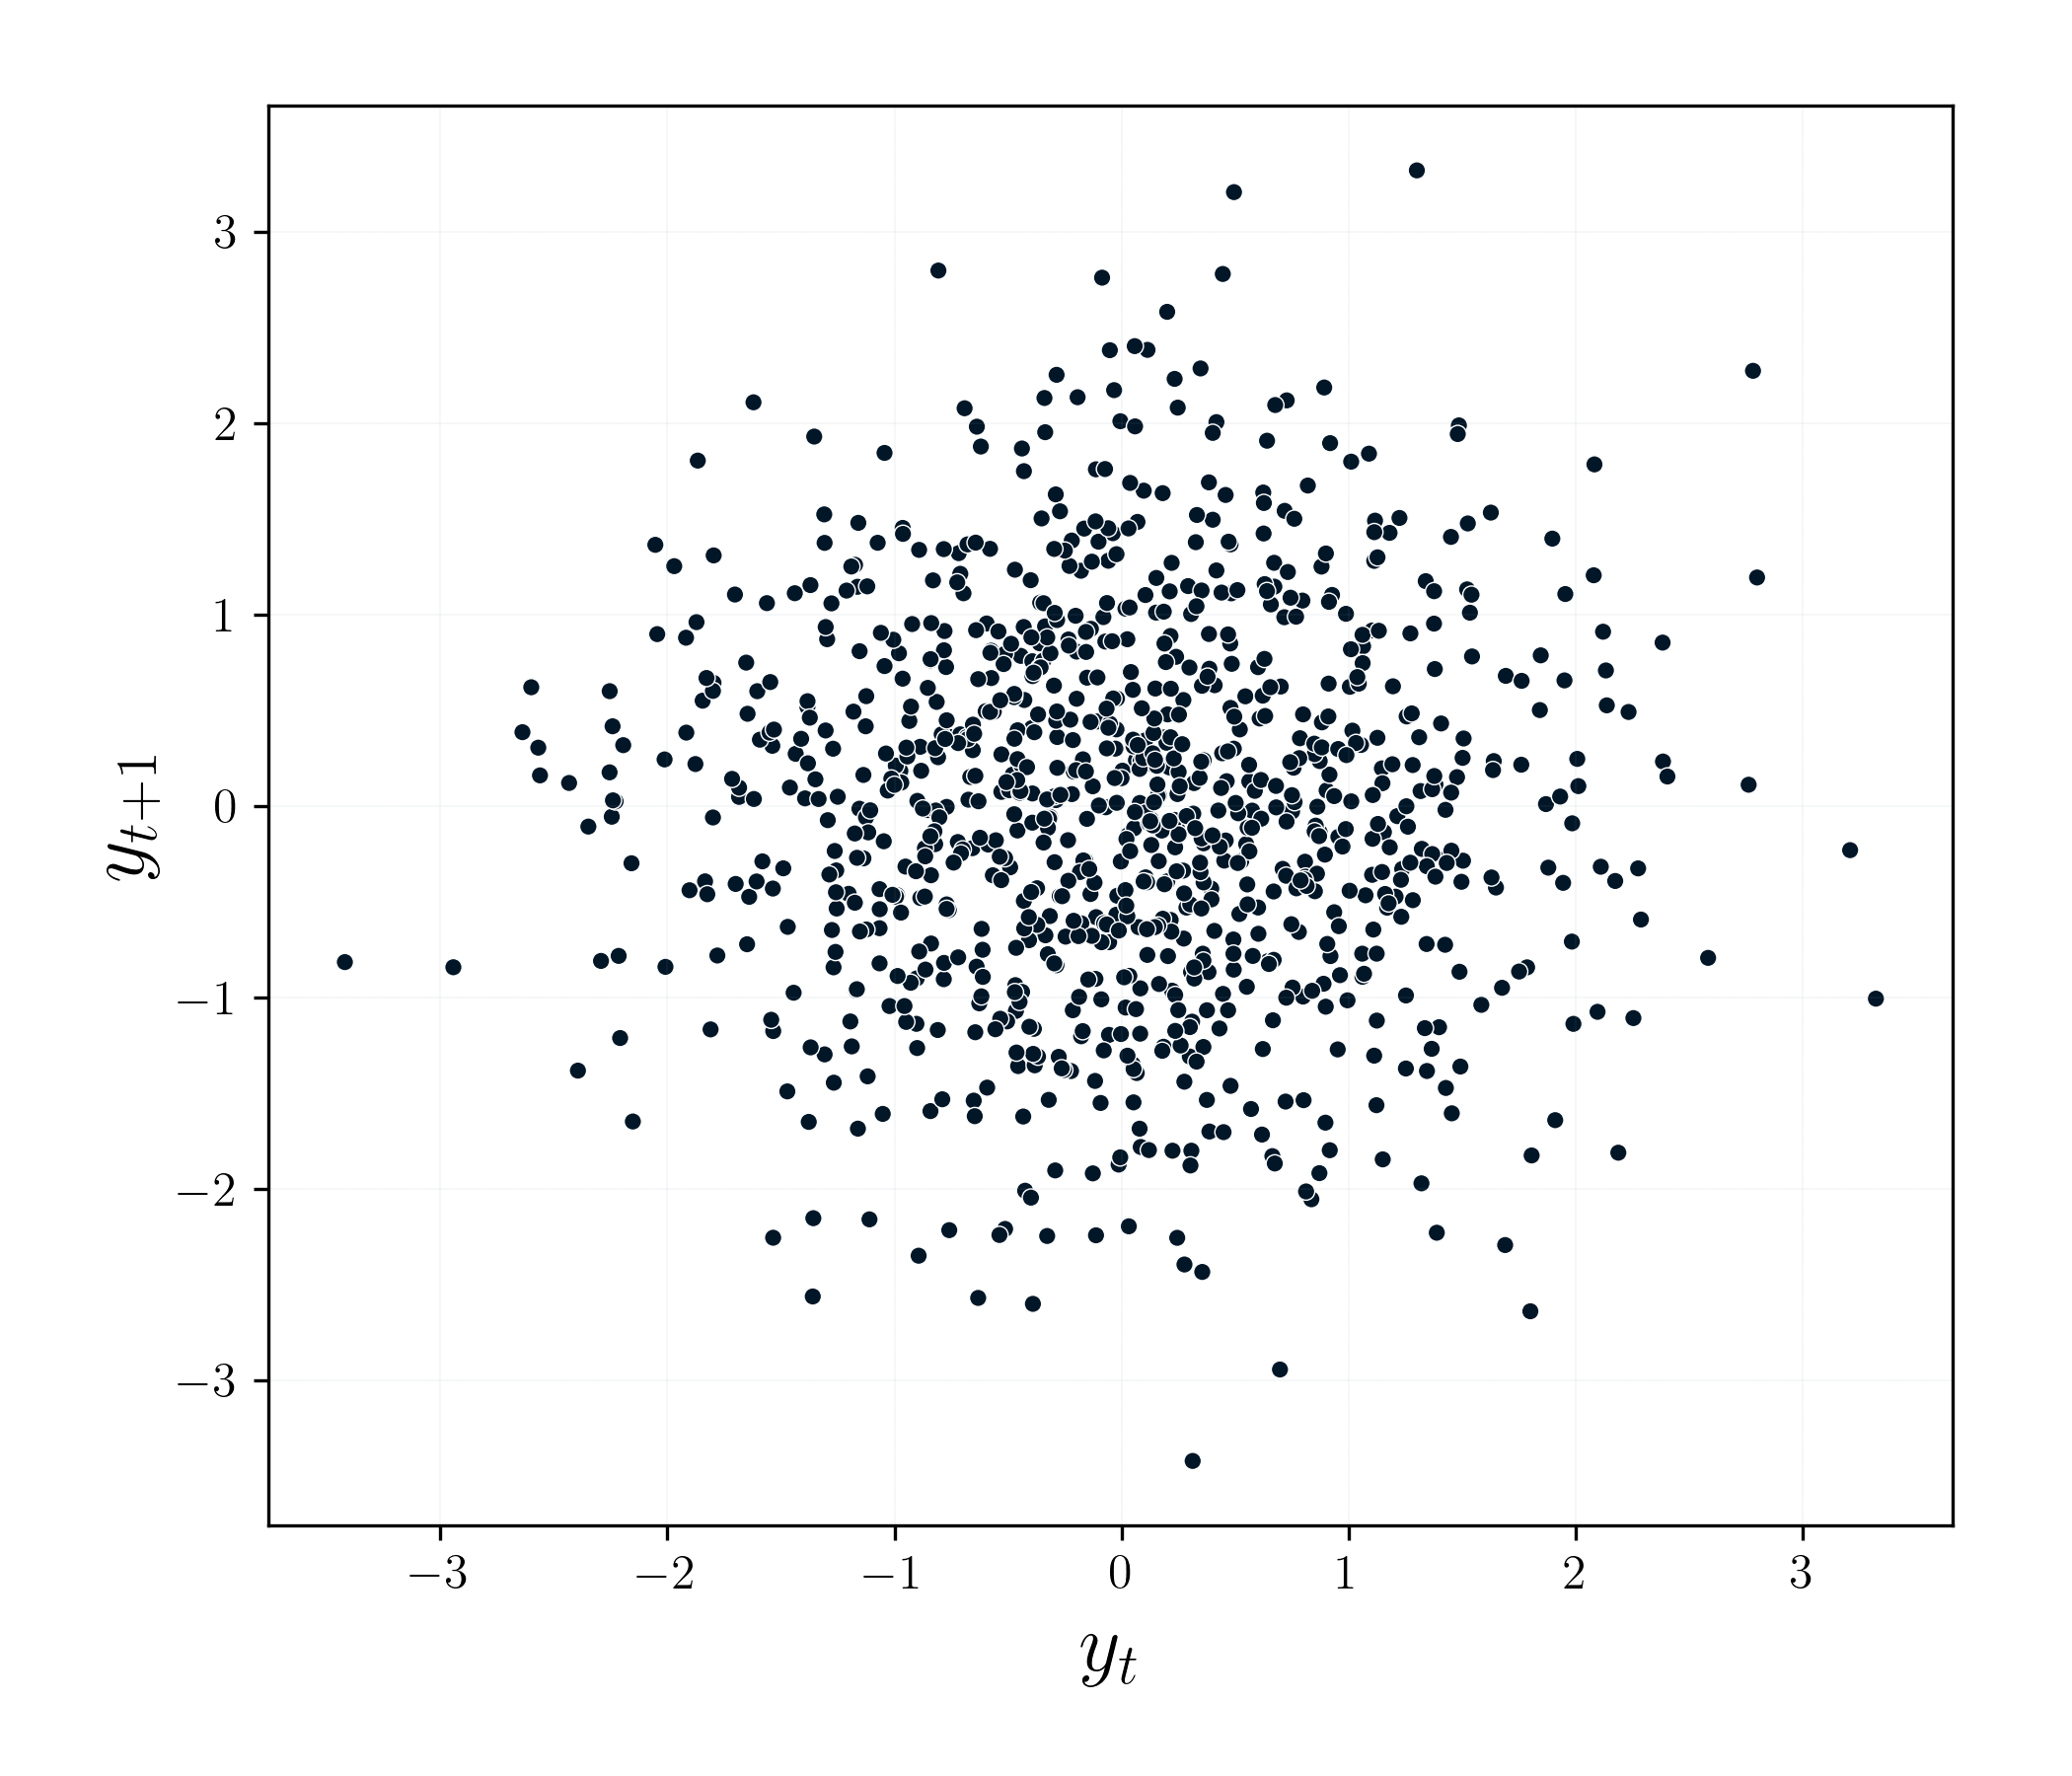
\includegraphics[width=1\textwidth, height=1\textheight, keepaspectratio]{random_series_lag_plot}
        \captionof{figure}{График задержек случайных величин, взятых из нормального 
        распределения с лагом $l = 1$. Построено программой по адресу 
        (листинг \ref{lst:time_series_lag_plot_random}).}
        \label{fig:lag_plot_random}
    \end{minipage}
\end{center}

График задержек помогает понять являются ли значения во временном ряду случайными. Если 
данные случайны, то на графике мы не увидим никакой определенной структуры. Однако 
если же данные не случайны, то на графике задержек можно будет увидеть ярко 
выраженную форму. 

Например на рисунке \ref{fig:lag_plot_wine} видно, что большая часть точек 
сгруппирована вокруг главной диагонали, что говорит о схожести продаж в соседние месяцы. 
В свою очередь на рисунке \ref{fig:lag_plot_random} нет никакой ярко выраженной 
структуры, что логично, так как это просто белый шум. \\

\paragraph{Матрица корреляций}

Еще одним широко распространенным методом графического анализа автокорреляции 
временного ряда является матрица корреляций (корреляционная матрица). Она отображает в 
себе корреляцию между всеми возможными заданными парами значений.

Рассмотрим матрицу корреляций на примере еженедельного общего объема продаж авокадо 
за 3 года (рис. \ref{fig:time_series_avocado}).

\begin{figure}[h!]
    \centering
    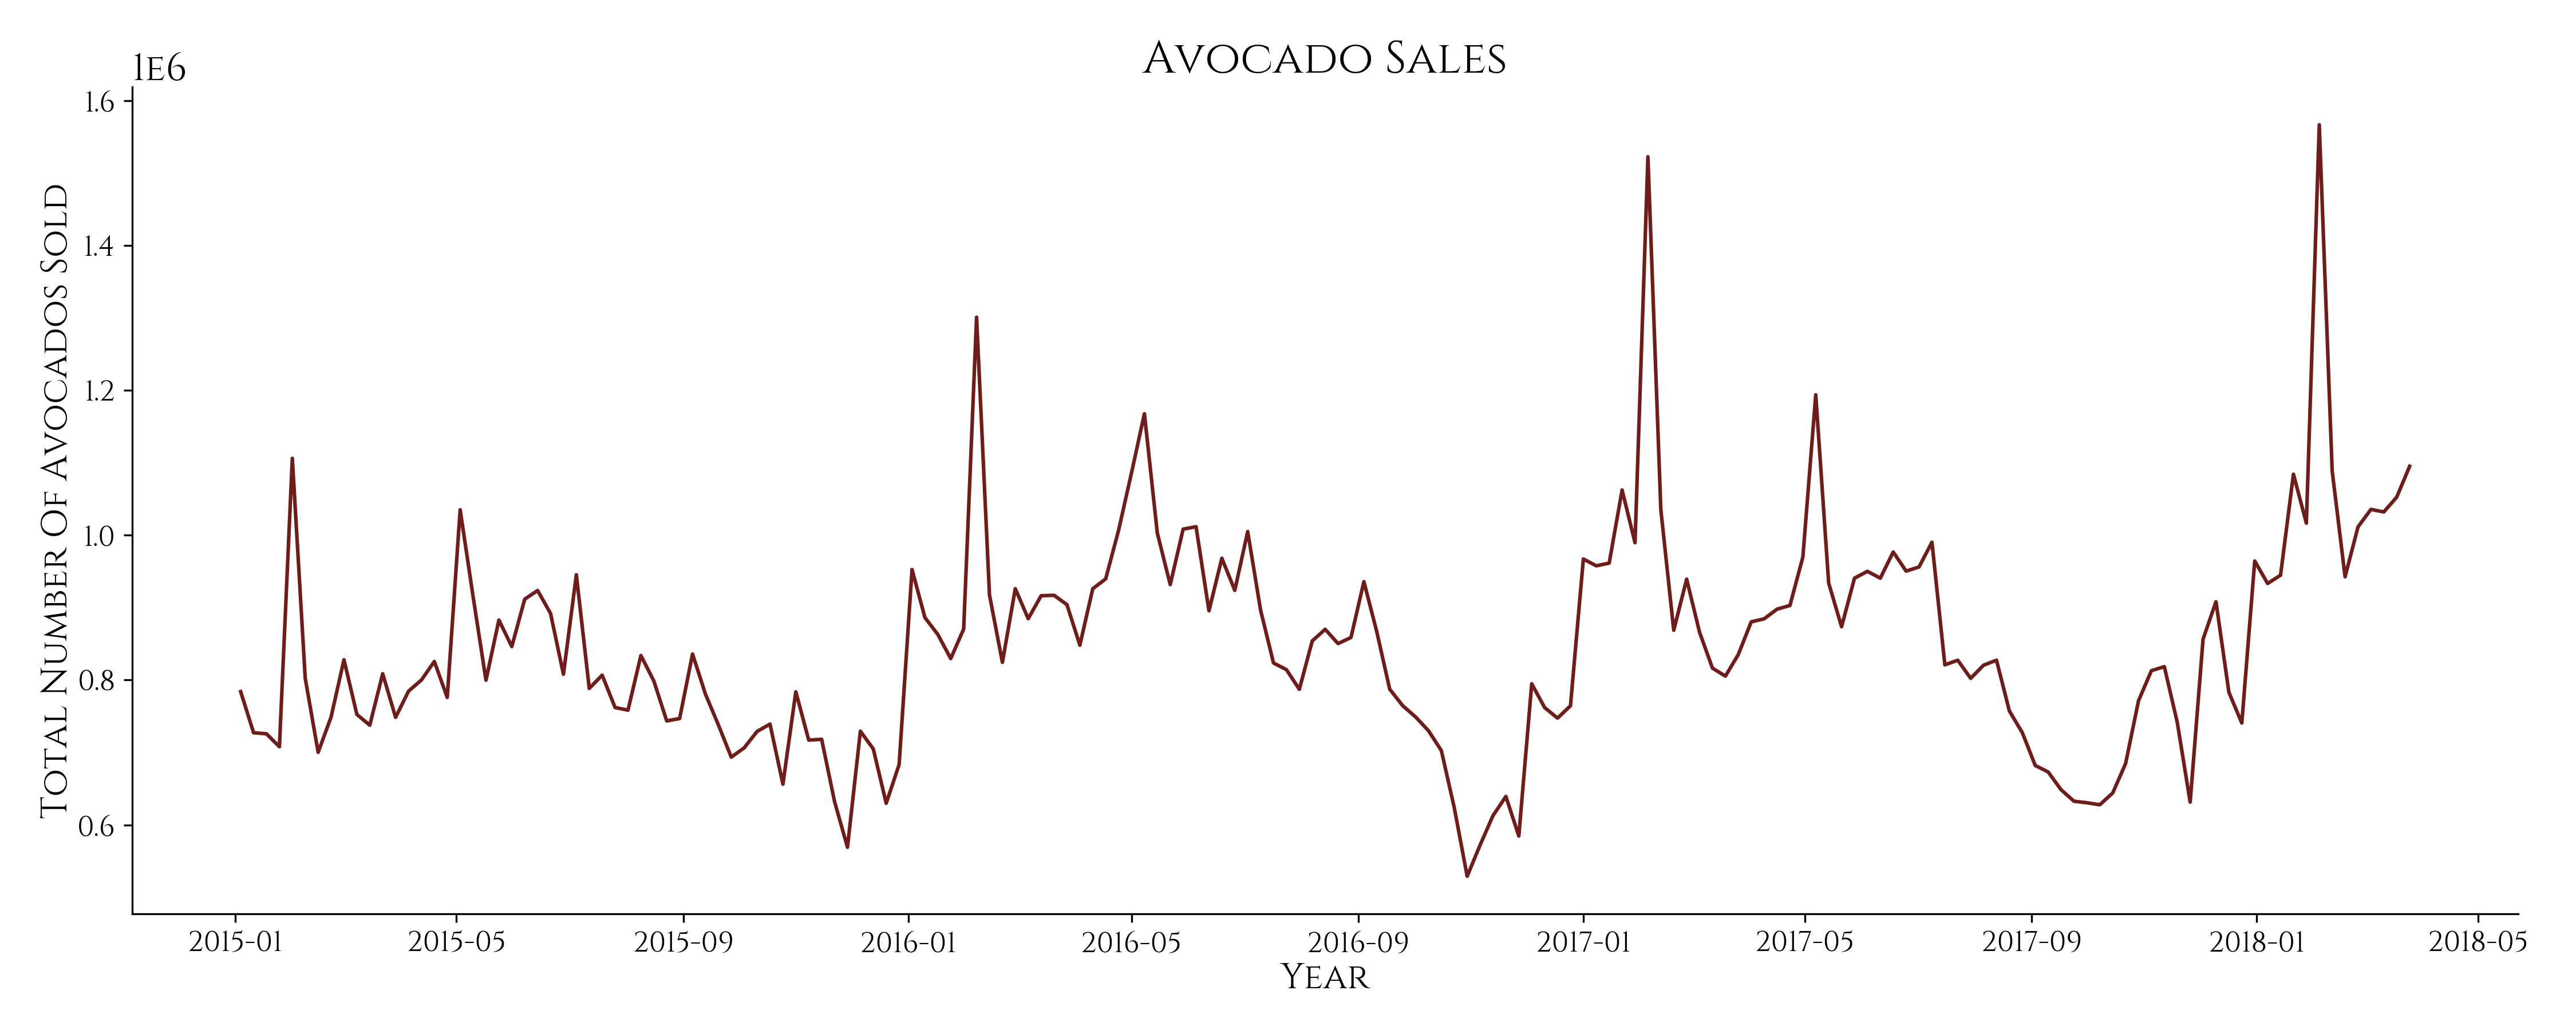
\includegraphics[width=1\textwidth, height=1\textheight, keepaspectratio]{time_series_example_avocado}
    \caption{Еженедельный объём продаж авокадо. Построено программой по адресу 
    (листинг \ref{lst:time_series_example_avocado}).}
    \label{fig:time_series_avocado}
\end{figure}

\begin{figure}[h!]
    \centering
    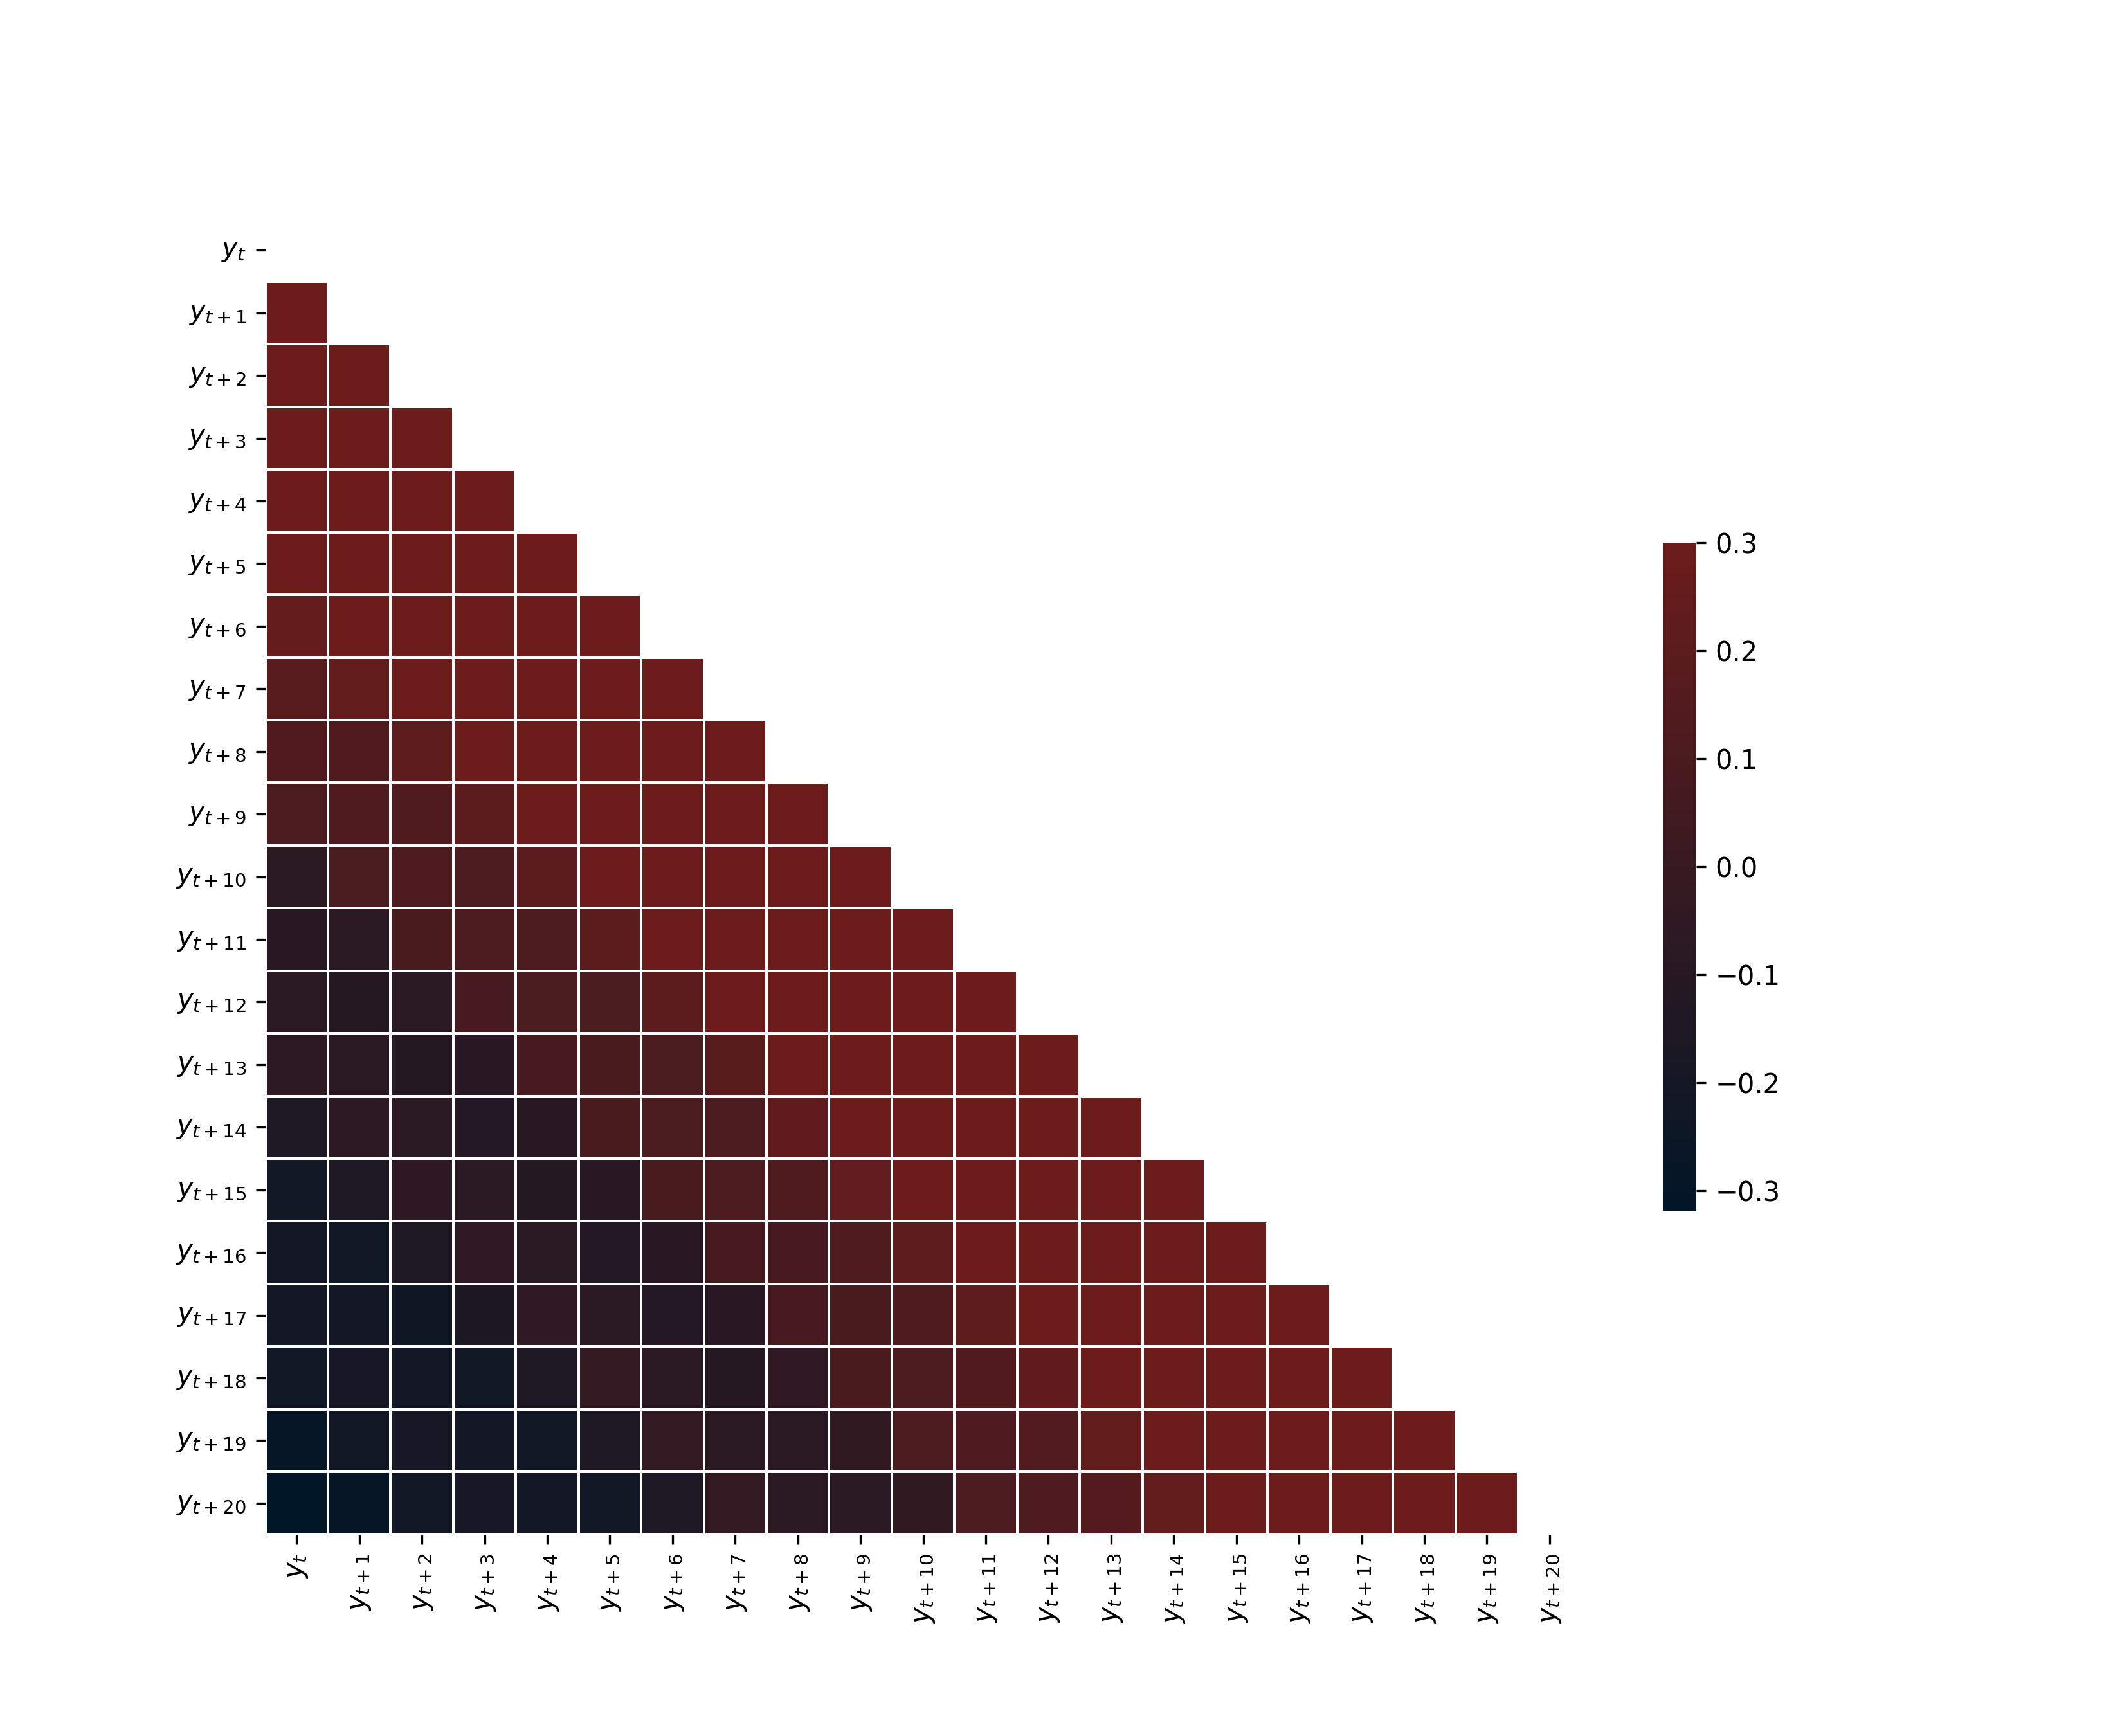
\includegraphics[width=1\textwidth, height=1\textheight, keepaspectratio]{correlation_matrix_avocado}
    \caption{Диагональная корреляционная матрица объема продаж авокадо. Построено 
    программой по адресу (листинг \ref{lst:correlation_matrix_avocado}).}
    \label{fig:correlation_matrix_avocado}
\end{figure}

\newpage

На рисунке \ref{fig:correlation_matrix_avocado} видно, что данные тем сильнее 
скоррелированны, чем ближе они находятся. Так например значения в соседних точках 
временного ряда $y_t$ и $y_{t+1}$ имеют корреляцию равную $0.3$, а $y_t$ и $y_{t+20}$, 
в свою очередь: $-0.3$.

\paragraph{Автокорреляционная функция}

График автокорреляции временного ряда от лага называется автокорреляционной 
функцией (ACF). Такой график также часто называют коррелограммой. По оси ординат на 
нём откладывается автокорреляция, а по оси абсцисс — размер лага $l$.

\begin{figure}[h!]
    \centering
    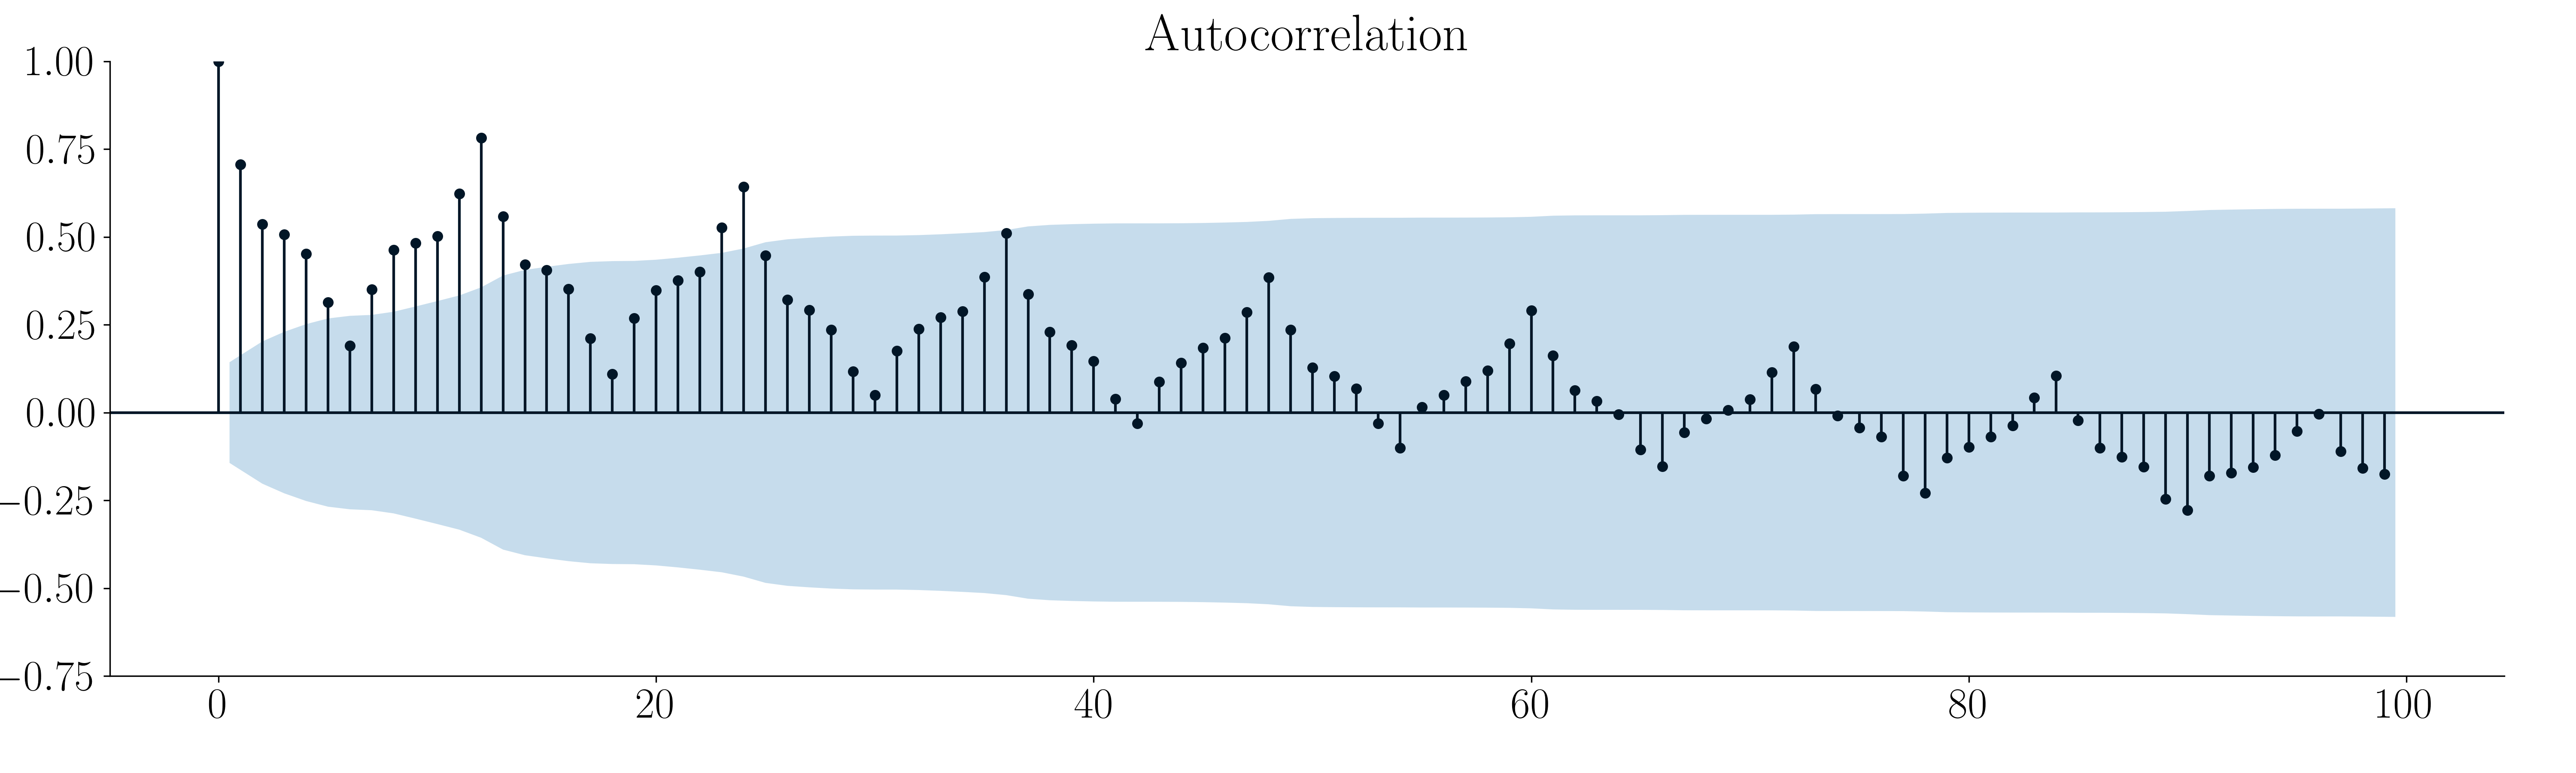
\includegraphics[width=1\textwidth, height=1\textheight, keepaspectratio]{acf_wine}
    \caption{Коррелограмма для объёма продаж красного вина в Австралии. Построено 
    программой по адресу (листинг \ref{lst:acf_wine}).}
    \label{fig:acf_wine}
\end{figure}

На рисунке \ref{fig:acf_wine} показан пример коррелограммы для исследуемых 
ранее данных о месячных продажах красного вина в Австралии 
(рисунок \ref{fig:time_series_wine}). На графике видно, что автокорреляция принимает 
большие значения в лагах, кратных сезонному периоду. Такой вид коррелограммы 
типичен для данных с выраженной сезонностью.

Стоит отметить, что автокорреляция может начать колебаться вокруг горизонтальной оси, 
соответствующей её нулевому значению, как это и произошло на рисунке \ref{fig:acf_wine}, 
а также, что автокорреляция в точке с лагом $l = 0$ всегда равна единице, 
так как в ней вычисляется корреляция значения ряда с самим собой.

Также на рисунке \ref{fig:acf_wine} изображён синий коридор вокруг горизонтальной оси. 
Это коридор значимости отличия корреляции от нуля. Фактически, все автокорреляции, 
которые изображены вне этого коридора, значимо отличаются от нуля.

\subsection{Стационарность}

\textbf{Определение} Если $\left\{y_t\right\}$ - стационарный временной ряд, то 
для любого $s$, распределение $(y_t, \dots, y_{t+s})$ не зависит от $t$ \cite{Forecasting_Hyndman}. \\

Таким образом, временные ряды с выраженным трендом или сезонностью не являются стационарными.
С другой стороны, белый шум, например, является стационарным - неважно в какой момент времени 
мы его рассмотрим, он будет выглядеть одинаково.

Иногда бывает затруднительно определить, является ли ряд стационарным. Временные ряды с 
непереодическими циклами (но без тренда или сезонности), например, не обязательно нестационарны, поскольку 
нельзя заранее предсказать положение максимумов и минимумов ряда.